%%%%%%%%%%%%%%%%%%%%%%%%%%%%%%%%%%%%%%%%%%%%%%%%%%%%%%%%%%%%%%%%%%%%%%%%%%%%%%%%
%2345678901234567890123456789012345678901234567890123456789012345678901234567890
%        1         2         3         4         5         6         7         8

\documentclass[letterpaper, 10 pt, conference]{ieeeconf}  % Comment this line out
                                                          % if you need a4paper
%\documentclass[a4paper, 10pt, conference]{ieeeconf}      % Use this line for a4
                                                          % paper

\IEEEoverridecommandlockouts                              % This command is only
                                                          % needed if you want to
                                                          % use the \thanks command
\overrideIEEEmargins
% See the \addtolength command later in the file to balance the column lengths
% on the last page of the document




% The following packages can be found on http:\\www.ctan.org
%\usepackage{graphics} % for pdf, bitmapped graphics files
%\usepackage{epsfig} % for postscript graphics files
%\usepackage{mathptmx} % assumes new font selection scheme installed
%\usepackage{times} % assumes new font selection scheme installed
%\usepackage{amsmath} % assumes amsmath package installed
%\usepackage{amssymb}  % assumes amsmath package installed
\usepackage{booktabs}
\usepackage{tikz}
\usepackage{pgfplots}
\pgfplotsset{compat=1.12}
\usepackage{multirow}
%\usepackage{draftwatermark}
%\SetWatermarkText{8====D}
\usetikzlibrary{calc,trees,positioning,arrows,chains,shapes.geometric,%
    decorations.pathreplacing,decorations.pathmorphing,shapes,%
    matrix,shapes.symbols}
    
    
\tikzset{
>=stealth',
  box/.style={
    rectangle, 
    rounded corners, 
    % fill=black!10,
    draw=black,  thick,
    text width=20em, 
    minimum height=1em, 
    minimum width=16em, 
    on chain},
     emptybox/.style={
    rectangle, 
    rounded corners, 
    % fill=black!10,
    draw=none,
    text width=18em, 
    minimum height=3em, 
    minimum width=16em, 
    on chain},
    mediumbox/.style={
    rectangle, 
    % fill=black!10,
    draw=black,  thick,
    text width=10em, 
    minimum height=2em, 
    minimum width=10em, 
    on chain},
  smallbox/.style={
    rectangle, 
    % fill=black!10,
    draw=red,
    on chain},
  line/.style={draw, thick, <-},
  element/.style={
    tape,
    top color=white,
    bottom color=blue!50!black!60!,
    minimum width=8em,
    draw=blue!40!black!90, very thick,
    text width=20em, 
    minimum height=3.5em, 
    text centered, 
    on chain},
  every join/.style={->, thick,shorten >=1pt},
  decoration={brace},
  tuborg/.style={decorate},
  tubnode/.style={midway, right=2pt},
}

\newcommand{\VtableDiagram}{ 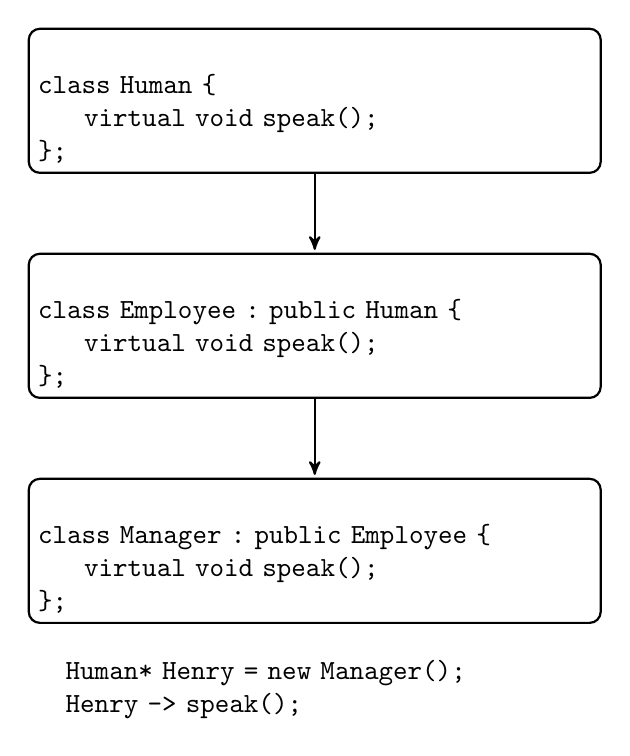
\begin{tikzpicture}
%  [node distance=.8cm,
[start chain=going below,]
\node[box, join] (Human) {
\begin{verbatim}
class Human {
     virtual void speak();
};\end{verbatim}
};
\node[box, join] (Employee) {
\begin{verbatim}
class Employee : public Human {
     virtual void speak();
};
\end{verbatim}
};
     
\node[box, join] (Manager) {
\begin{verbatim}
class Manager : public Employee {
     virtual void speak();
};
\end{verbatim}
};

\node[emptybox, below of=Manager,node distance =  15pt] (Code) {
\begin{verbatim}
Human* Henry = new Manager();
Henry -> speak();
\end{verbatim}
};


\end{tikzpicture} }

\title{\LARGE \bf
Power Consumption For Mobile System Security
}

%\author{ \parbox{3 in}{\centering Huibert Kwakernaak*
%         \thanks{*Use the $\backslash$thanks command to put information here}\\
%         Faculty of Electrical Engineering, Mathematics and Computer Science\\
%         University of Twente\\
%         7500 AE Enschede, The Netherlands\\
%         {\tt\small h.kwakernaak@autsubmit.com}}
%         \hspace*{ 0.5 in}
%         \parbox{3 in}{ \centering Pradeep Misra**
%         \thanks{**The footnote marks may be inserted manually}\\
%        Department of Electrical Engineering \\
%         Wright State University\\
%         Dayton, OH 45435, USA\\
%         {\tt\small pmisra@cs.wright.edu}}
%}


\begin{document}

\maketitle
\thispagestyle{empty}
\pagestyle{empty}


\begin{abstract}

The past decade has seen a sharp increase in the number of security vulnerabilities in modern smartphones. Modern defenses such as Control Flow Integrity (CFI) and Virtual Table Verification (VTV) are popularly being used on large scale systems but have not yet reached mobile technologies, such as ARM, the processor on which almost all leading smartphones run. 

While performance is certainly important, a key concern that drives adoption of a security mechanism on mobile devices is its effect on battery life. This paper discusses the energy impact of two popular security mechanisms on mobile devices (CFI and VTV). We use the most widely used implementations that have been downstreamed to the popular open sourced LLVM compiler. This paper therefore measures the increased power consumption of using CFI and the Vtable verification mechanism on an ARM device. By repeatedly running tests from the SPEC benchmark suite on a battery driven power source we were able to measure each defense's added power consumption along with its overall performance. Our results indicate a relative increase in effective power consumption of each defense on ARM based devices.
\end{abstract}

%%%%%%%%%%%%%%%%%%%%%%%%%%%%%%%%%%%%%%%%%%%%%%%%%%%%%%%%%%%%%%%%%%%%%%%%%%%%%%%%
\section{INTRODUCTION}

Over the past decade we have witnessed a massive evolution in system exploits and defenses for those exploits. While stronger defenses are constantly being built, attackers find new innovative means to counter them. Most of these attacks are based on vulnerabilities found in code built in type unsafe languages like C and C++ and Objective C.

A popular defense presently being explored is Control Flow Integrity (CFI), first proposed by Abadi et Al~\cite{abadi}. The purpose of CFI is to ensure that the execution of a program stays within the bounds of its control flow graph (CFG). Since it's inception in 2005, there have been a variety of CFI mechanisms proposed (see~\cite{trop},~\cite{mocfi},~\cite{picfi},~\cite{safed}). These mechanisms differ in their granularity in terms of types of checks and their frequency. For instance, the original CFI paper talks about protecting return addresses by maintaining a shadow stack in memory; IFCC by google checks only forward edges for sanitizing indirect calls; k-bouncer leverages only the branch history of the last few indirect calls found in modern x86 processors.~\cite{trop}

Security is often seen as a second class citizen when it comes to embedded devices. While adoption of new mitigation practices is slow on regular operating systems, they are seen to be even slower on embedded operating systems. This can be seen by the slow adoption of various defensive mechanisms such as SE Linux and inbuilt firewalls by Google's Android and Apple's iOS, the leading brands of smartphones today. This is primarily due to the fact that with limited resources, all modern smartphones tend to provide a vast number of features with high performance; thereby squeezing the underlying hardware to provide services at its highest capability. However, due to an increasing dependency on smartphones, and the large amount of personal and private information being amassed on these devices; they have become a major target for attackers.

Over the past few years, several vulnerabilities were found in both Android and iOS system libraries that have been exploited to gain root privileges on those devices. Among these one of the most noteworthy vulnerabilities were found in the libstagefright library, a media playback library in the Android operating system. These allowed an attacker to remotely get root privilege and perform arbitrary code execution on the target device.

Most CFI mechanisms have been proposed for Intel based hardware. Very little attention has been given to ARM devices. Most smartphones today run on the ARM architecture <numbers>. The ARM architecture is a natural choice for mobile technology due to their use of the Reduced Instruction Set Architecture (RISC).

While performance is certainly important, a critical factor for the adoption of CFI on ARM is its effect on battery life. It is essential for hardware and software vendors to have an understanding of the battery power consumption of any mechanism, in order to make a rounded decision on its employment.

In this paper, we plan to test both the performance and energy consumption of LLVM's CFI as well as V-Table Verification mechanism.

We measure performance based on the run-time generated by the respective SPEC CPU 2006 benchmarks and the energy consumption through the relative rate of consumption of power from the battery pack.

Through this paper we present the following:
\begin{itemize}
\item A simple yet trustworthy testing mechanism for measuring power consumption of any security mechanism on mobile devices.
\item Relative power consumption of control flow integrity on the ARMv7 architecture.
\item Performance costs of different mechanisms on the ARMv7 architecture.
\end{itemize}

This paper is organized in the following sections:
(II) Background, where we go over various modern attack vectors, mitigation mechanisms and power measurement practices.
(III) Methodology, Here we explain our testing mechanism and hardware in detail.
(IV) Performance Measurements and Results: Where present the results of our tests in detail, and
(V) Discussion and Future Work, where we discuss possible improvements and extensions that we intend to explore.

\section{BACKGROUND}

%%%% VIRTUAL FUNCTION CLASS HIERARCHY %%%%%%%%%%%%
\begin{figure}[t]
\label{vtable}
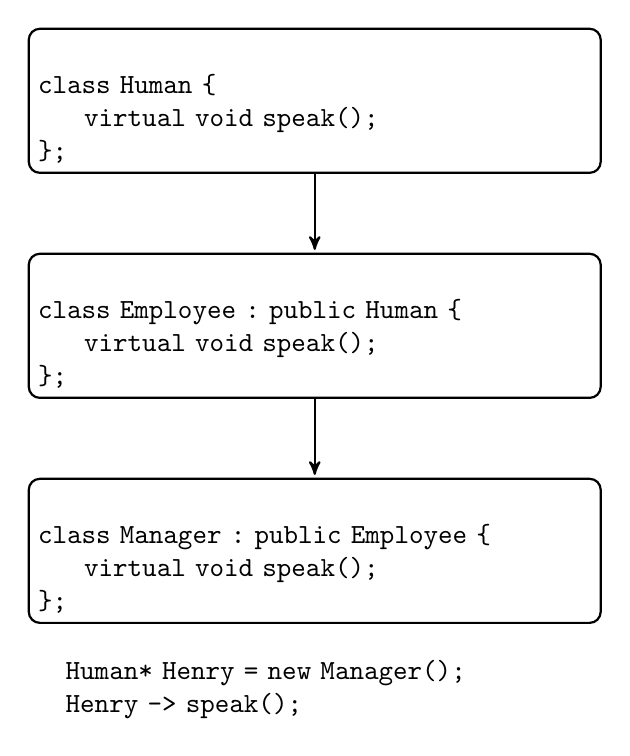
\begin{tikzpicture}
%  [node distance=.8cm,
[start chain=going below,]
\node[box, join] (Human) {
\begin{verbatim}
class Human {
     virtual void speak();
};\end{verbatim}
};
\node[box, join] (Employee) {
\begin{verbatim}
class Employee : public Human {
     virtual void speak();
};
\end{verbatim}
};
     
\node[box, join] (Manager) {
\begin{verbatim}
class Manager : public Employee {
     virtual void speak();
};
\end{verbatim}
};

\node[emptybox, below of=Manager,node distance =  15pt] (Code) {
\begin{verbatim}
Human* Henry = new Manager();
Henry -> speak();
\end{verbatim}
};


\end{tikzpicture}
\caption{Example: Class Hierarchy with Virtual Function}
\end{figure}
%%%%%%%%%%%%%%%%%%%%%%%%%%%%%%%%%%%%%%%%%%%%%%%%%%

This section provides a brief understanding of the various defenses that have been tested in this paper along with a portion on power measurement practices. We divide them into three categories, namely: Control Flow Integrity,Virtual Table Verification and Power Measurement Practices.

\subsection{Control Flow Integrity}
The advent of Execute-Only memory, also known as Data Execution Prevention (DEP), had removed the possibility of mounting simple code injection attacks. Attackers could no longer inject code directly into the heap or program stack and change the Instruction Pointer to execute that code. Without being able to arbitrarily use their own code, attackers began manipulate the instruction pointer to utilize existing code sequences (called gadgets) in order to mount their attack. This is known as Return Oriented Programming (ROP); where the goal for the attacker is usually to stitch together a sequence of gadgets in order to make a privileged system call (i.e., a return-to-libc attack)~\cite{gadgets}. With the right gadget(s), Return Oriented Programming has been proven to be Turing complete~\cite{turing}.

Early defenses against ROP attacks were to increase entropy of the code by means of randomization. However, this is still open to other kinds of attacks~\cite{aslr}. For instance, ASLR (Address Space Layout Randomization) randomizes the location of gadgets in memory preventing an attacker from finding or propagating ROP attacks based on memory locations. However, ASLR and other such software diversity mechanisms are vulnerable to memory leak related exploits~\cite{failaslr}. Also, as seen recently, software diversity on mobile operating systems is often weakly enforced~\cite{zygote}.

Control flow integrity adds a stronger, code level defense mitigating any incorrect call that is not per the expected control flow. CFI therefore involves maintaining a predetermined CFG (usually obtained during compile time) and adding checks to ensure the valid flow of control at runtime. A fine grained CFI policy essentially checks three components: 
Return Addresses 
Indirect Calls 
and Indirect Jumps 

Strongly enforced CFI policies can completely stop all ROP attacks.

\subsection{Virtual Table Verification}

%%%% NORMAL V-CALL %%%%%%%%%%%%%%%%%%%%%%%
\begin{figure}
\label{normal-vcall}
\begin{tikzpicture}
%  [node distance=.8cm,
[start chain=going below,]

\node[smallbox, below left of=Code, node distance = 23 pt, left, blue] (vptr) {
VPTR
};

\node[mediumbox, right of=vptr,node distance=130pt, blue] (Vtable) {
Human Vtable \\
$\rightarrow$ Human: speak() \\
$\rightarrow$  Employee: speak() \\
$\rightarrow$  Manager: speak() \\
};

\node[mediumbox, below right of=vptr, node distance = -17pt] (Henry) {
Henry              
};

%\draw [->] (vptr) -- (Vtable);

\draw [->, blue] (vptr) to [out=10,in=170] (Vtable);
\end{tikzpicture}
\caption{Example: Normal Virtual Call}
\end{figure}
%%%%%%%%%%%%%%%%%%%%%%%%%%%%%%%%%%%%%%%%%%%%%%%%%%

%%%% V-CALL ATTACK DIAGRAM %%%%%%%%%%%%%%%%%%%%%%%
\begin{figure}
\label{attacker}
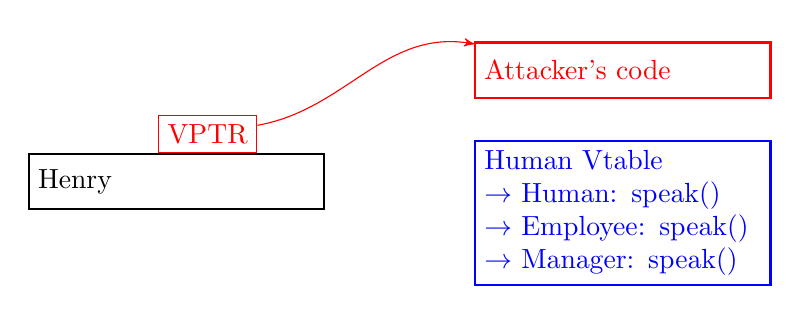
\begin{tikzpicture}
[start chain=going below,]

\node[smallbox, red] (vptr) {
VPTR
};

\node[mediumbox, right of=vptr,node distance=150pt, blue] (Vtable) {
Human Vtable \\
$\rightarrow$ Human: speak() \\
$\rightarrow$  Employee: speak() \\
$\rightarrow$  Manager: speak() \\
};

\node[mediumbox, below right of=vptr, node distance = -16pt] (Henry) {
Henry              
};

\node[mediumbox, above of=Vtable, node distance = 80pt, red] (Devil) {
Attacker's code
};

%\draw [->] (vptr) -- (Vtable);

\draw [->, red] (vptr) to [out=10,in=170] (Devil);

  \end{tikzpicture}
\caption{Example: Virtual Call Attack}
\end{figure}
%%%%%%%%%%%%%%%%%%%%%%%%%%%%%%%%%%%%%%%%%%%%%%%%%%

With CFI policies essentially blocking all ROP attacks; adversaries have started leveraging object oriented language constructs in languages like C++. Vtable hijacking recently has become a popular mechanism to break the integrity of code. V-Table hijacking, as the name suggests, takes advantage of the C++ mechanism for handling dynamic type casting (also known as dynamic dispatch)~\cite{coop}.

To manage dynamic dispatch, every C++ object has a hidden pointer to a virtual table (or v-table). This vtable contains references to all the functions that the object can possibly be cast to. Then at runtime, based on the type of object the variable is holding; the correct call is made. 

Figure~\ref{vtable} above explains the functioning of C++ dynamic dispatch. The pseudo code defines three classes: Employee, Human and Manager; where Manager inherits from Employee which in turn inherits from Human. The code below it shows an overloaded call fulfilled through the C++ dynamic dispatch mechanism. When calling Henry's speak function, the system de-references the object's vtable and finds a pointer to the Manager class' speak function. This function pointer is further de-referenced to make the correct call at run-time.

By taking advantage of code errors (e.g., use after free bugs), the attacker can essentially change the v-table pointer to point to an attacker controlled table (as shown in Figure~\ref{attacker}). This could be a table that is a) crafted by the attacker himself, b) the base of another existing table in memory or c) the middle of a pre-existing table.

To counter such V-Table hijacking attacks, Jang et. al suggested the use of a vtable verification mechanism (VTV)~\cite{safed}. V-Table verification involves checking indirect jumps to functions for validity. In order to perform this check, most mechanisms encode class hierarchy information in all virtual functions~\cite{vtrust}. Before making the indirect call the compiler adds verification code to ensure that the address stored in the register is a valid one as per the encoded data.

\subsection{Power Measurement Practices}
There are various practices for measuring power on systems. They are broadly categorized as: a) Online b) Offline and c) Simulated.
Power can be measured online by tracking the per-rail power consumption of every component on the device. This entails maintaining an understanding of every component and subcomponent on the underlying hardware (eg: CPU, RAM, gyroscope, network card etc). Each component is perceived to have a variety of hardware states and each of these states is associated with an estimated power metric. The accuracy of this mechanism is therefore completely dependent on the fine grained division of the various states as well as the frequency of probing the components for their states. This method also emits a large amount of asynchronous data that needs to be correlated and further analyzed. While many existing tools do this calculation after the tests have been completed; some perform them live at the cost of extra CPU cycles; for instance, Qualcomm's Trepn does live analysis of real time data while Zhang et. al's PowerTutor performs this calculation after~\cite{powertutor}. Online power consumption also suffers from the problem of self-consumption; i.e., it incurs a cost both in CPU cycles and energy while measuring power.

Offline Power is measured externally from the device. This involves connecting the device to an external source of power and getting an analysis of the consumption based on actual values. It therefore treats the device as a black-box and all calculations are carried out externally based on real values. This mechanism is highly accurate as it measures the true power consumed by the device. It does however incur a higher monetary cost for building the external set up.

Power may also be measured via a simulated mechanism. Simulated power calculation is carried out by a host system that has an integrated understanding of the hardware in question. Simulated mechanisms associate a power cost of every single machine instruction. While executing the binary they simply put together the cost of each executed instruction. Simulated mechanisms are not widely used due to inability to provide very accurate results. Not many simulated power tools exist as they involve a very deep modeling of the system and cannot accurately portray multi-threading and caching.

In this paper, we use the offline approach to measuring power consumption on the mobile hardware as it is by far the most accurate way to measure relative power consumption.

\section{EXPERIMENTAL METHODOLOGY}

%%%% SPEC TABLE %%%%%%%%%%%%%%%%%%%%%%%%%%%%%%%%%%%%%%%%%%%%%%%%%%%%%%%%
\begin{table*}[t]
\centering
\caption{Virtual Call Related Statistics for SPEC Benchmarks}
\label{spec}
\bgroup
\def\arraystretch{1.5}
\begin{tabular}{l|llll|ll}
            & \multicolumn{4}{l|}{Runtime Profiling}                       & \multicolumn{2}{l|}{Static Count} \\ \hline
            & No. instructions & Indirect calls & Indirect jumps & Return  & Vtable           & Vcall          \\ \hline
471.omnetpp & 22 billion       & 11.19\%        & 18.63\%        & 70.18\% & 127              & 1431           \\
473.astar   & 15 billion       & 32.95\%        & 0.07\%         & 66.98\% & 2                & 0              \\ \hline
\end{tabular}
\egroup
\end{table*}
%%%%%%%%%%%%%%%%%%%%%%%%%%%%%%%%%%%%%%%%%%%%%%%%%%%%%%%%%%%%%%%%%%%%%%%%

%%%% RESULTS TABLE %%%%%%%%%%%%%%%%%%%%%%%%%%%%%%%%%%%%%%%%%%%%%%%%%%%%%
\begin{table*}
\centering
\caption{Relative Power Consumption and Run-time of CFI and VTV}
\label{results-table}
\bgroup
\def\arraystretch{1.5}
\begin{tabular}{l|l|ll|lll|lll}
\hline
Test Description                                                                                                            & Iteration & \multicolumn{2}{l}{\begin{tabular}[c]{@{}l@{}}Time Until\\ Crash (minutes)\end{tabular}} & \multicolumn{2}{l|}{\begin{tabular}[c]{@{}l@{}}Estimated Power\\ Consumption (Watts)\end{tabular}} & Increase & \multicolumn{2}{l|}{\begin{tabular}[c]{@{}l@{}}Run-time \\ (seconds)\end{tabular}} & Increase \\ \hline
                                                                                                                            &           & OFF                                         & ON                                         & OFF                                              & ON                                              &          & OFF                                      & ON                                      &          \\ \hline
\multirow{4}{*}{\begin{tabular}[c]{@{}l@{}}Benchmark: omnetpp\\ Mechanism: VTV\\ Repetitions per iteration: 2\end{tabular}} & 1         & 342                                         & 321                                        & 14.211                                           & 15.14                                           & 6.54\%   & 10970                                    & 11134                                   & 1.49\%   \\
                                                                                                                            & 2         & 333                                         & 333                                        & 14.595                                           & 14.595                                          & 0.00\%   & 10891                                    & 11212                                   & 2.95\%   \\
                                                                                                                            & 3         & 334                                         & 328                                        & 14.551                                           & 14.817                                          & 1.83\%   & 10932                                    & 11244                                   & 2.85\%   \\
                                                                                                                            & 4         & 336                                         & 324                                        & 14.464                                           & 15                                              & 3.71\%   & 11003                                    & 11092                                   & 0.81\%   \\ \hline
Average                                                                                                                     &           &                                             &                                            & 14.455                                           & 14.888                                          & 3.02\%   &                                          &                                         & 2.03\%   \\ \hline
\multirow{3}{*}{\begin{tabular}[c]{@{}l@{}}Benchmark: astar\\ Mechanism: CFI\\ Repetitions per iteration: 3\end{tabular}}   & 1         & 322                                         & 312                                        & 15.093                                           & 15.577                                          & 3.21\%   & 15386                                    & 15407                                   & 0.14\%   \\ \cline{2-10} 
                                                                                                                            &           &                                             &                                            &                                                  &                                                 &          &                                          &                                         &          \\
                                                                                                                            &           &                                             &                                            &                                                  &                                                 &          &                                          &                                         &          \\ \hline
\end{tabular}
\egroup
\end{table*}
%%%%%%%%%%%%%%%%%%%%%%%%%%%%%%%%%%%%%%%%%%%%%%%%%%%%%%%%%%%%%%%%%%%%%%%%

%%%% BAR GRAPH %%%%%%%%%%%%%%%%%%%%%%%%%%%%%%%%%%%%%%%%%%%%%%%%%%%%%%%%%
\begin{figure}
\caption{Relative Power Consumption of CFI and VTV}
\label{fig-results-bar}
\input{results.txt}
\end{figure}
%%%%%%%%%%%%%%%%%%%%%%%%%%%%%%%%%%%%%%%%%%%%%%%%%%%%%%%%%%%%%%%%%%%%%%%%

For this experiment we used an Inforce Snapdragon single-board computer: INF6410 with the following specifications: 
\begin{enumerate}
\item Qualcomm Snapdragon S4 Pro APQ8064 compliant with the ARMv7-MP instruction set
\item Quad core Krait, 1.7GHz
\item 2 GB on-board DDR3
\item An externally powered SSD drive
\item Ubuntu Linux 14.10 (Linaro utopic developer build)
\end{enumerate}

We chose this set-up as it forms the bare minimum specs on any modern mobile device sold as of date. In order to reduce external factors from effecting our results, we used an externally powered SSD, disabled network access to the devices, disconnected all external input sources (keyboard) and disabled the output to the display. All tests were run through a system startup script; we used cron to start our test script.

The external battery source was made up of 12 AA Nickel-Metal Hydride (NiMH) batteries (12 per run) connected in parallel to a voltage stabilizing buck (switching regulator). NiMH batteries have a stable voltage over capacity drain until they hit maximum capacity after which there a sharp decline in voltage essentially powering off the device.

Our initial experiments on an Alkaline based source proved to be unstable as Alkaline sources have a steadily reducing output voltage over capacity. At about half the capacity of the battery pack, the voltage would drop to below the usable capacity causing our experiment to fail.

In order to get accurate results, for each experiment, we first selected a single test from the benchmark suite and ran it till it drained the battery pack. We then determined the number of complete test runs that could be performed.

We then ran the baseline and the implemented mechansim one after another with only the selected number of runs of one test. Once the benchmarks were complete the board would be in idle state from some time until it died. We had a cron job that logged the current time after every 60 seconds; this gave us a fairly accurate measure on what time the battery pack was completely drained. We then took the absolute time of death for each experiment and performed further analysis on the results to obtain the average power difference between the two sets.

To reduce bias due relative capacity loss over consecutive charge cycles, we used two identical sets of twelve Alkaline batteries that were alternated for each run. Thus, both baseline and secure code executions ran at exactly the same number of charge cycles.

SPEC benchmarks astar and omnetpp (Why?) \\
Compilation problems - vcall and normal cfi \\

\section{PERFORMANCE MEASUREMENTS AND RESULTS}



Virtual Table Verification
In order to test the power and performance cost of LLVM's V-Table Verification mechanism, we compiled the SPEC CPU 2006 benchmark suite test: Omnetpp with it. After sampling the number of stable runs on the battery pack; we considered two complete executions of the ref input set to be adequate. We ran four iterations of this test and obtained a 2.03\% increase in CPU usage (measured in running time) and a 3.02\% increase in power consumption (measured in Watts).\\

Control Flow Integrity
To test the power and performance cost of the full suite of LLVM's Control Flow Integrity mechanism (CFI + VTV), we compiled the SPEC CPU 2006 benchmark suite test: Astar with it. Unfortunately, due to time constraints, we were only able to run one iteration of this experiment; however, our results are none the less in the expected range. We calculated a 0.14\% increase in CPU usage (measured in running time) and a 3.21\% increase in power consumption (measured in Watts).\\


\section{Conclusion and Future Work}

In this paper we have experimentally shown a fair relative increase in both performance and power consumption of LLVM's downstreamed Control Flow Integrity and V-Table Verification mechanisms on ARMv7 based devices. This information can be utilized by any manufacturer or provider of mobile technology who wishes to introduce any of the aforementioned defense mechanisms on their product line. We also suggest the experimental set-up used in this paper as it is the most accurate way of measuring the power consumption of any system level change.

While our results are fairly definitive, we believe that, given time we can further bolster our claim by running a greater number of iterations. We also think that by adding more defenses to our tests, we can eventually get a broad spectrum understanding of the power consumption of different system security mechanisms on mobile platforms.


\addtolength{\textheight}{-12cm}   % This command serves to balance the column lengths
                                  % on the last page of the document manually. It shortens
                                  % the textheight of the last page by a suitable amount.
                                  % This command does not take effect until the next page
                                  % so it should come on the page before the last. Make
                                  % sure that you do not shorten the textheight too much.


%%%%%%%%%%%%%%%%%%%%%%%%%%%%%%%%%%%%%%%%%%%%%%%%%%%%%%%%%%%%%%%%%%%%%%%%%%%%%%%%

\bibliographystyle{plain}
\nocite{*}
\bibliography{bibliography}

\end{document}
